\documentclass[12pt]{article}
%\usepackage{setspace}
%\usepackage{gensymb}
%\doublespacing
%\singlespacing
%\usepackage{graphicx}
%\usepackage{amssymb}
%\usepackage{relsize}
\usepackage[cmex10]{amsmath}
%\usepackage{amsthm}
%\interdisplaylinepenalty=2500
%\savesymbol{iint}
%\usepackage{txfonts}
%\restoresymbol{TXF}{iint}
%\usepackage{wasysym}
\usepackage{amsthm}
%\usepackage{iithtlc}
\usepackage{mathrsfs}
\usepackage{txfonts}
\usepackage{stfloats}
\usepackage{bm}
\usepackage{cite}
\usepackage{cases}
\usepackage{subfig}
%\usepackage{xtab}
\usepackage{longtable}
\usepackage{multirow}
%\usepackage{algorithm}
%\usepackage{algpseudocode}
\usepackage{enumitem}
\usepackage{mathtools}
\usepackage{steinmetz}
\usepackage{tikz}
\usepackage{circuitikz}
\usepackage{verbatim}
\usepackage{tfrupee}
\usepackage[breaklinks=true]{hyperref}
%\usepackage{stmaryrd}
\usepackage{tkz-euclide} % loads  TikZ and tkz-base
%\usetkzobj{all}
\usepackage{atbegshi}
\AtBeginDocument{\AtBeginShipoutNext{\AtBeginShipoutDiscard}}
\usetikzlibrary{calc,math}
\usepackage{listings}
    \usepackage{color}                                            %%
    \usepackage{array}                                            %%
    \usepackage{longtable}                                        %%
    \usepackage{calc}                                             %%
    \usepackage{multirow}                                         %%
    \usepackage{hhline}                                           %%
    \usepackage{ifthen}                                           %%
  %optionally (for landscape tables embedded in another document): %%
    \usepackage{lscape}     
\usepackage{multicol}
\usepackage{chngcntr}
%\usepackage{enumerate}

%\usepackage{wasysym}
%\newcounter{MYtempeqncnt}
\DeclareMathOperator*{\Res}{Res}
\renewcommand{\baselinestretch}{2}
\renewcommand\thesection{\arabic{section}}
\renewcommand\thesubsection{\thesection.\arabic{subsection}}
\renewcommand\thesubsubsection{\thesubsection.\arabic{subsubsection}}

%\renewcommand\thesectiondis{\arabic{section}}
%\renewcommand\thesubsectiondis{\thesectiondis.\arabic{subsection}}
%\renewcommand\thesubsubsectiondis{\thesubsectiondis.\arabic{subsubsection}}

% correct bad hyphenation here
\hyphenation{op-tical net-works semi-conduc-tor}
\def\inputGnumericTable{}                                 %%

\lstset{
%language=C,
frame=single, 
breaklines=true,
columns=fullflexible
}
\begin{document}
\newtheorem{theorem}{Theorem}[section]
\newtheorem{problem}{Problem}
\newtheorem{proposition}{Proposition}[section]
\newtheorem{lemma}{Lemma}[section]
\newtheorem{corollary}[theorem]{Corollary}
\newtheorem{example}{Example}[section]
\newtheorem{definition}[problem]{Definition}
%\newtheorem{thm}{Theorem}[section] 
%\newtheorem{defn}[thm]{Definition}
%\newtheorem{algorithm}{Algorithm}[section]
%\newtheorem{cor}{Corollary}
\newcommand{\BEQA}{\begin{eqnarray}}
\newcommand{\EEQA}{\end{eqnarray}}
\newcommand{\define}{\stackrel{\triangle}{=}}

\bibliographystyle{IEEEtran}
\bibliographystyle{ieeetr}
\providecommand{\mbf}{\mathbf}
\providecommand{\pr}[1]{\ensuremath{\Pr\left(#1\right)}}
\providecommand{\qfunc}[1]{\ensuremath{Q\left(#1\right)}}
\providecommand{\sbrak}[1]{\ensuremath{{}\left[#1\right]}}
\providecommand{\lsbrak}[1]{\ensuremath{{}\left[#1\right.}}
\providecommand{\rsbrak}[1]{\ensuremath{{}\left.#1\right]}}
\providecommand{\brak}[1]{\ensuremath{\left(#1\right)}}
\providecommand{\lbrak}[1]{\ensuremath{\left(#1\right.}}
\providecommand{\rbrak}[1]{\ensuremath{\left.#1\right)}}
\providecommand{\cbrak}[1]{\ensuremath{\left\{#1\right\}}}
\providecommand{\lcbrak}[1]{\ensuremath{\left\{#1\right.}}
\providecommand{\rcbrak}[1]{\ensuremath{\left.#1\right\}}}
\theoremstyle{remark}
\newtheorem{rem}{Remark}
\newcommand{\sgn}{\mathop{\mathrm{sgn}}}
%\providecommand{\abs}[1]{\left\vert#1\right\vert}
\providecommand{\res}[1]{\Res\displaylimits_{#1}} 
%\providecommand{\norm}[1]{\left\lVert#1\right\rVert}
%\providecommand{\norm}[1]{\lVert#1\rVert}
\providecommand{\mtx}[1]{\mathbf{#1}}
%\providecommand{\mean}[1]{E\left[ #1 \right]}
\providecommand{\fourier}{\overset{\mathcal{F}}{\rightleftharpoons}}
%\providecommand{\hilbert}{\overset{\mathcal{H}}{\rightleftharpoons}}
\providecommand{\system}{\overset{\mathcal{H}}{\longleftrightarrow}}
	%\newcommand{\solution}[2]{\textbf{Solution:}{#1}}
\newcommand{\solution}{\noindent \textbf{Solution: }}
\newcommand{\cosec}{\,\text{cosec}\,}
\providecommand{\dec}[2]{\ensuremath{\overset{#1}{\underset{#2}{\gtrless}}}}
\newcommand{\myvec}[1]{\ensuremath{\begin{pmatrix}#1\end{pmatrix}}}
\newcommand{\mydet}[1]{\ensuremath{\begin{vmatrix}#1\end{vmatrix}}}
\let\vec\mathbf
\begin{center}
\title{\textbf{Straight Lines}}
\date{\vspace{-5ex}} %Not to print date automatically
\maketitle
\end{center}
\setcounter{page}{1}
\section*{11$^{th}$ Maths - Chapter 10}
This is Problem-12 from Exercise 10.4
\begin{enumerate}
    \item Find the equation of the line passing through the point of intersection of the lines $4x + 7y - 3 = 0$ and $2x - 3y + 1 = 0$ that has equal intercepts on the axes.\\
    \solution \\
    Given lines can be written in the form of \begin{align}
        \Vec{n}^{\top}\Vec{x} = c
    \end{align}
   \\Therefore,\\
		\begin{align}
       \myvec{4&7}\vec{x}=3
       \label{eq:2}
   \end{align} 
   \begin{align}
       \myvec{2&-3}\vec{x}=-1
       \label{eq:3}
   \end{align}\\
   Now, line equation that has equal intercepts on the axes is
   \begin{align}
       \myvec{1 & 1}\Vec{x}=c
       \label{eq:4}
   \end{align}
   Solving equations \eqref{eq:2} and \eqref{eq:3}
		\\augumented matrix is
 \begin{align}
    \myvec{4&7&3\\2&-3&-1}\\
    \xleftrightarrow{R_1 \leftarrow 4 R_1}
    \myvec{1&\frac{7}{4}&\frac{3}{4}\\2&-3&-1}
    \xleftrightarrow{R_2 \leftarrow R_2 - 2R_1}
    \myvec{1&\frac{7}{4}&\frac{3}{4}\\0&\frac{-13}{2}&\frac{-5}{2}}\\
    \xleftrightarrow{R_2 \leftarrow \frac{-2}{13}R_2}
    \myvec{1&\frac{7}{4}&\frac{3}{4}\\0&1&\frac{5}{13}}
    \xleftrightarrow{R_1 \leftarrow R_1-\frac{7}{4}R_2}
    \myvec{1&0&\frac{1}{13}\\0&1&\frac{5}{13}}
\end{align}
Therfore, \begin{align}    
\vec{x} = \myvec{\frac{1}{13}\\\frac{5}{13}}
\end{align}
Also this point lies on the equation \eqref{eq:4}\\
\begin{center}
\begin{align}
    \myvec{1 & 1}\myvec{\frac{1}{13}\\\frac{5}{13}} = c\\
    \frac{1}{13}+\frac{5}{13} = c
    \end{align}
    \end{center}
    Therefore, the equation is \begin{align}
        \myvec{1&1}\Vec{x}=\frac{6}{13}
    \end{align}
\begin{figure}[h]
    \centering
    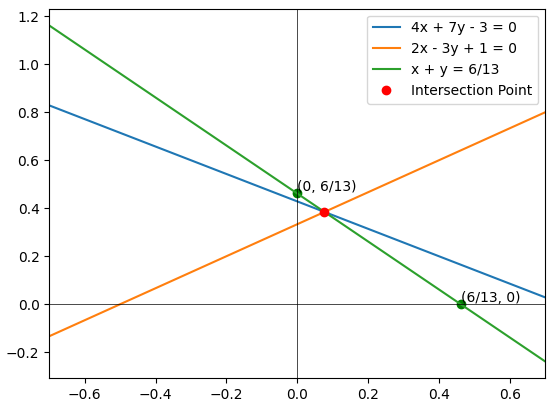
\includegraphics[width=\columnwidth]{figs/straightline.png}
    \caption{Straight Lines}
    \label{fig:enter-label}
\end{figure}
\end{enumerate}
\end{document}
